\subsection{Cuestionario 4}

\subsubsection{Pre-juego}
\begin{questions}
	
	\question ¿Cuál es tu edad?
	_______________________
	Respuesta: El público en su mayoría que ha respondido la encuesta se encuentra entre los 21 y 25 años de edad y algunas personas entre los 30 y 40 años.
	
	\question ¿Cuál es tú nivel de estudios?
	\begin{checkboxes}
		\choice Básica
		\choice Media superior
		\choice Superior
		\choice Doctorado o maestría
	\end{checkboxes}

\begin{figure}
	\centering
	\caption{Gráfica de nivel de estudios}
	\label{fig:pre01}
	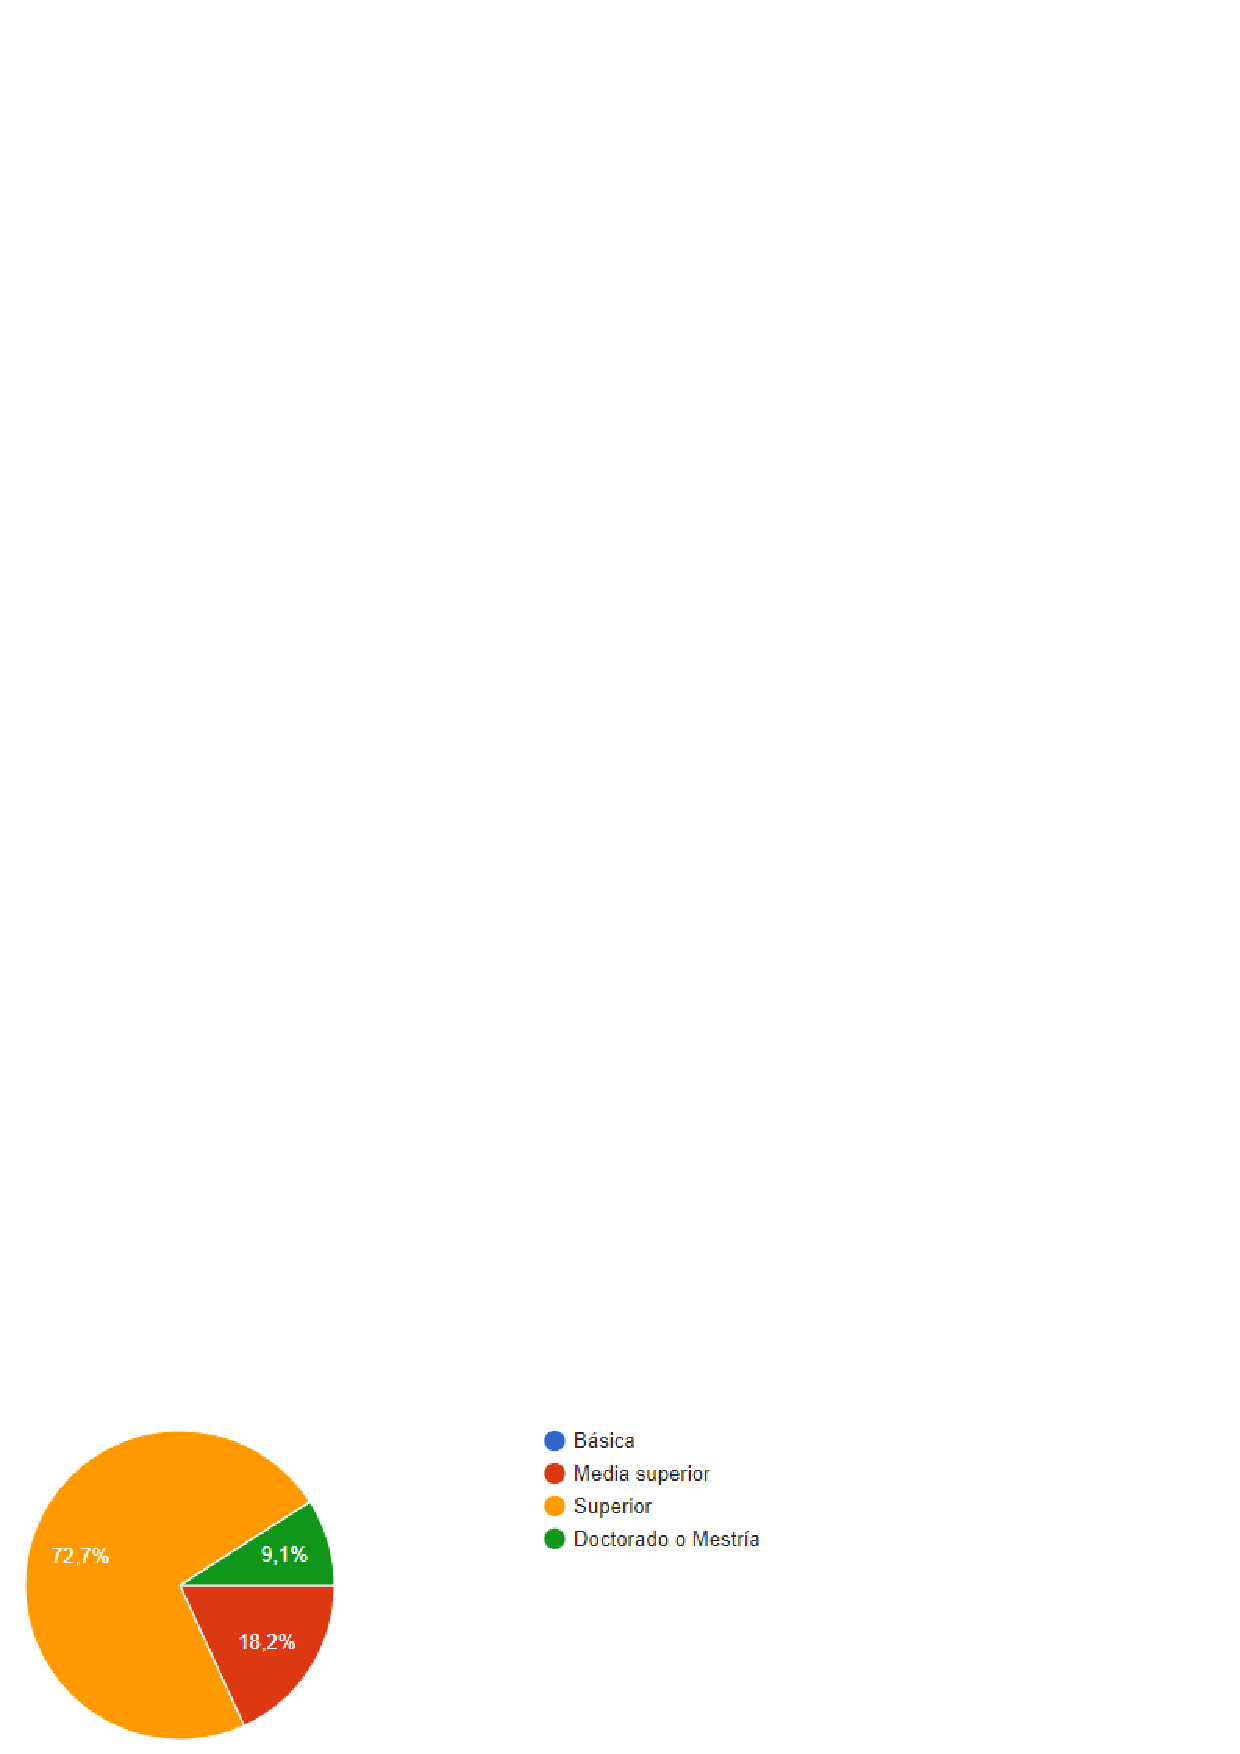
\includegraphics[width=0.5\textwidth]{imagenes\que\pre01}
\end{figure}

	
	\question ¿Qué es lo primero que piensas cuando te dicen "cultura de México"?
	\begin{checkboxes}
		\choice Comida
		\choice Arquitectura o lugares
		\choice Vestimenta
		\choice Música
		\choice Idioma	
	\end{checkboxes}

\begin{figure}
	\centering
	\caption{Gráfica de cultura de México}
	\label{fig:pre02}
	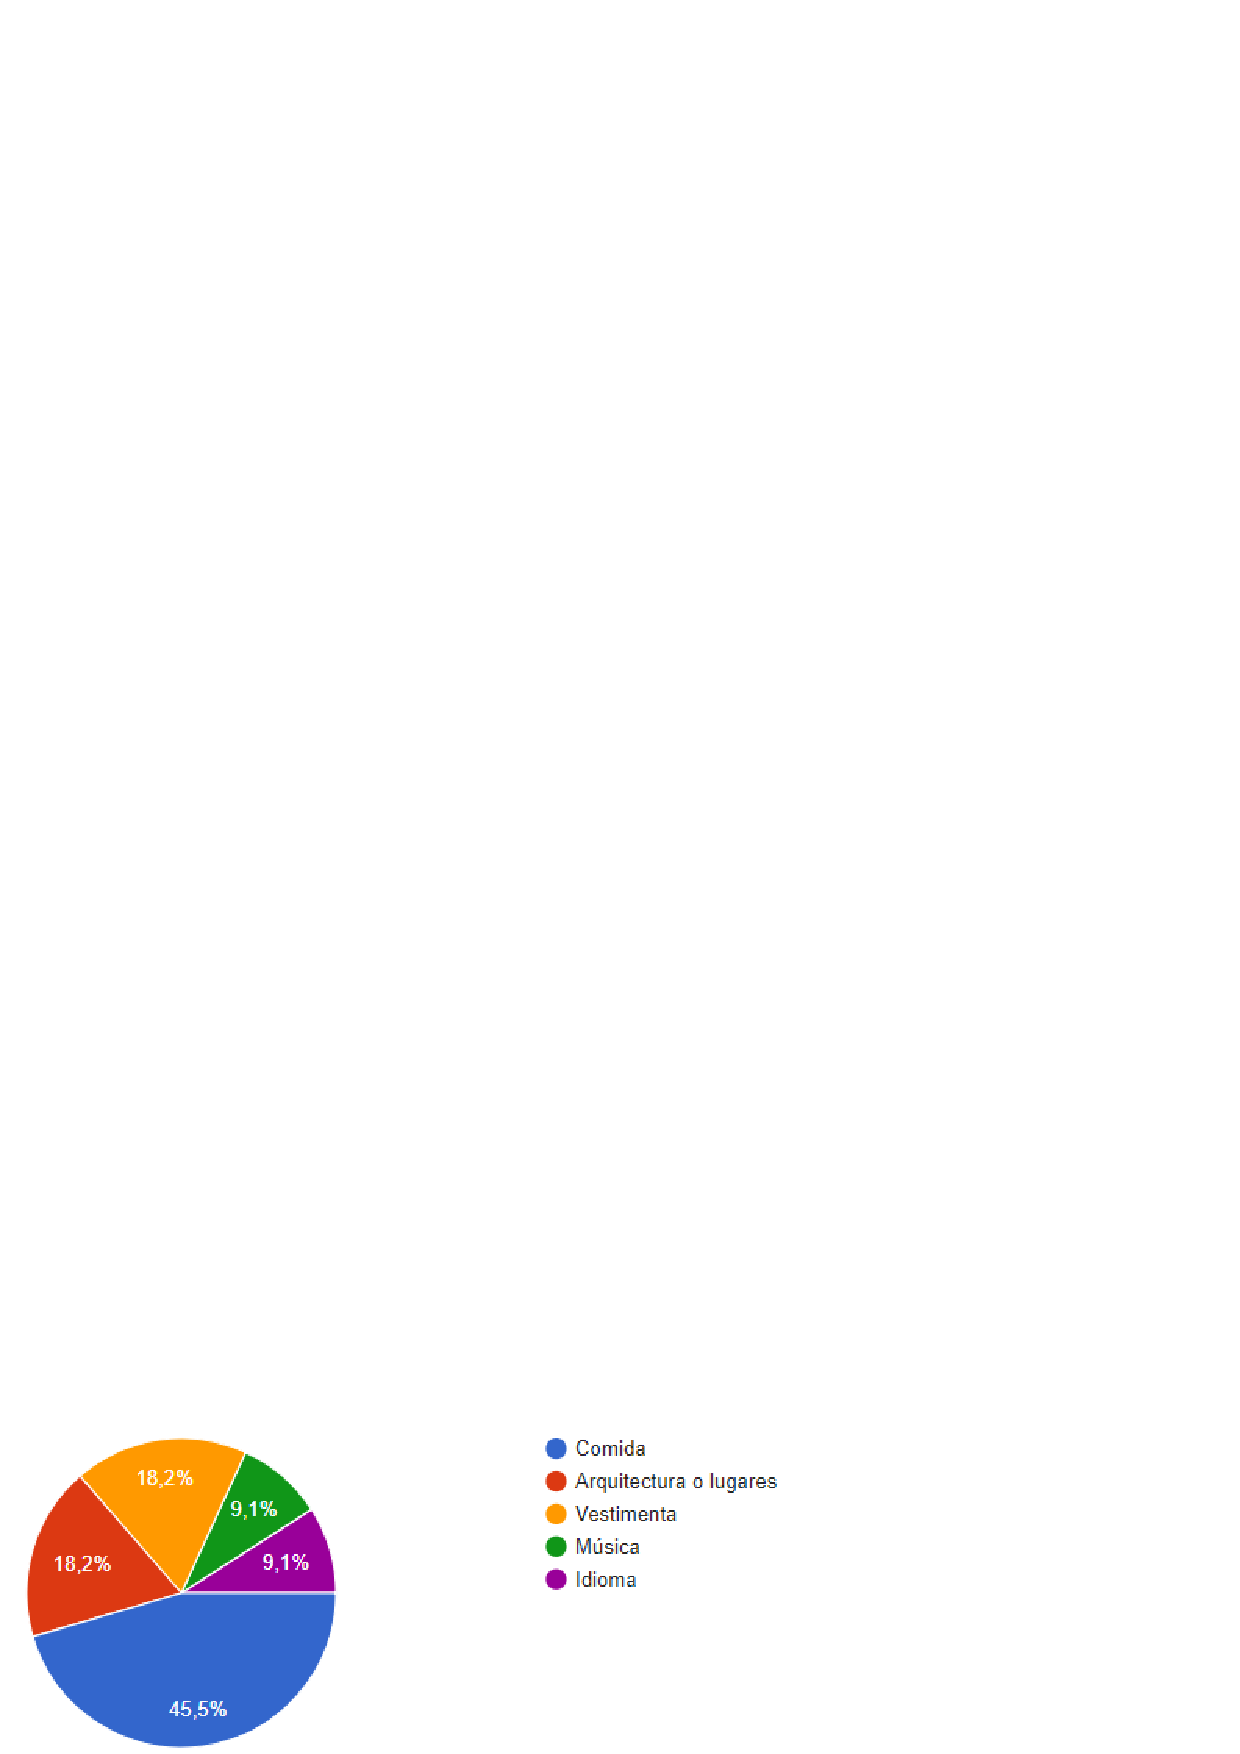
\includegraphics[width=0.5\textwidth]{imagenes\que\pre02}
\end{figure}

	
	\question ¿Por qué motivos visitas lugares históricos?
	\begin{checkboxes}
		\choice Escuela
		\choice Trabajo
		\choice Evento especial
		\choice Interés propio
		\choice Otro?
	\end{checkboxes}

\begin{figure}
	\centering
	\caption{Gráfica de lugares históricos}
	\label{fig:pre03}
	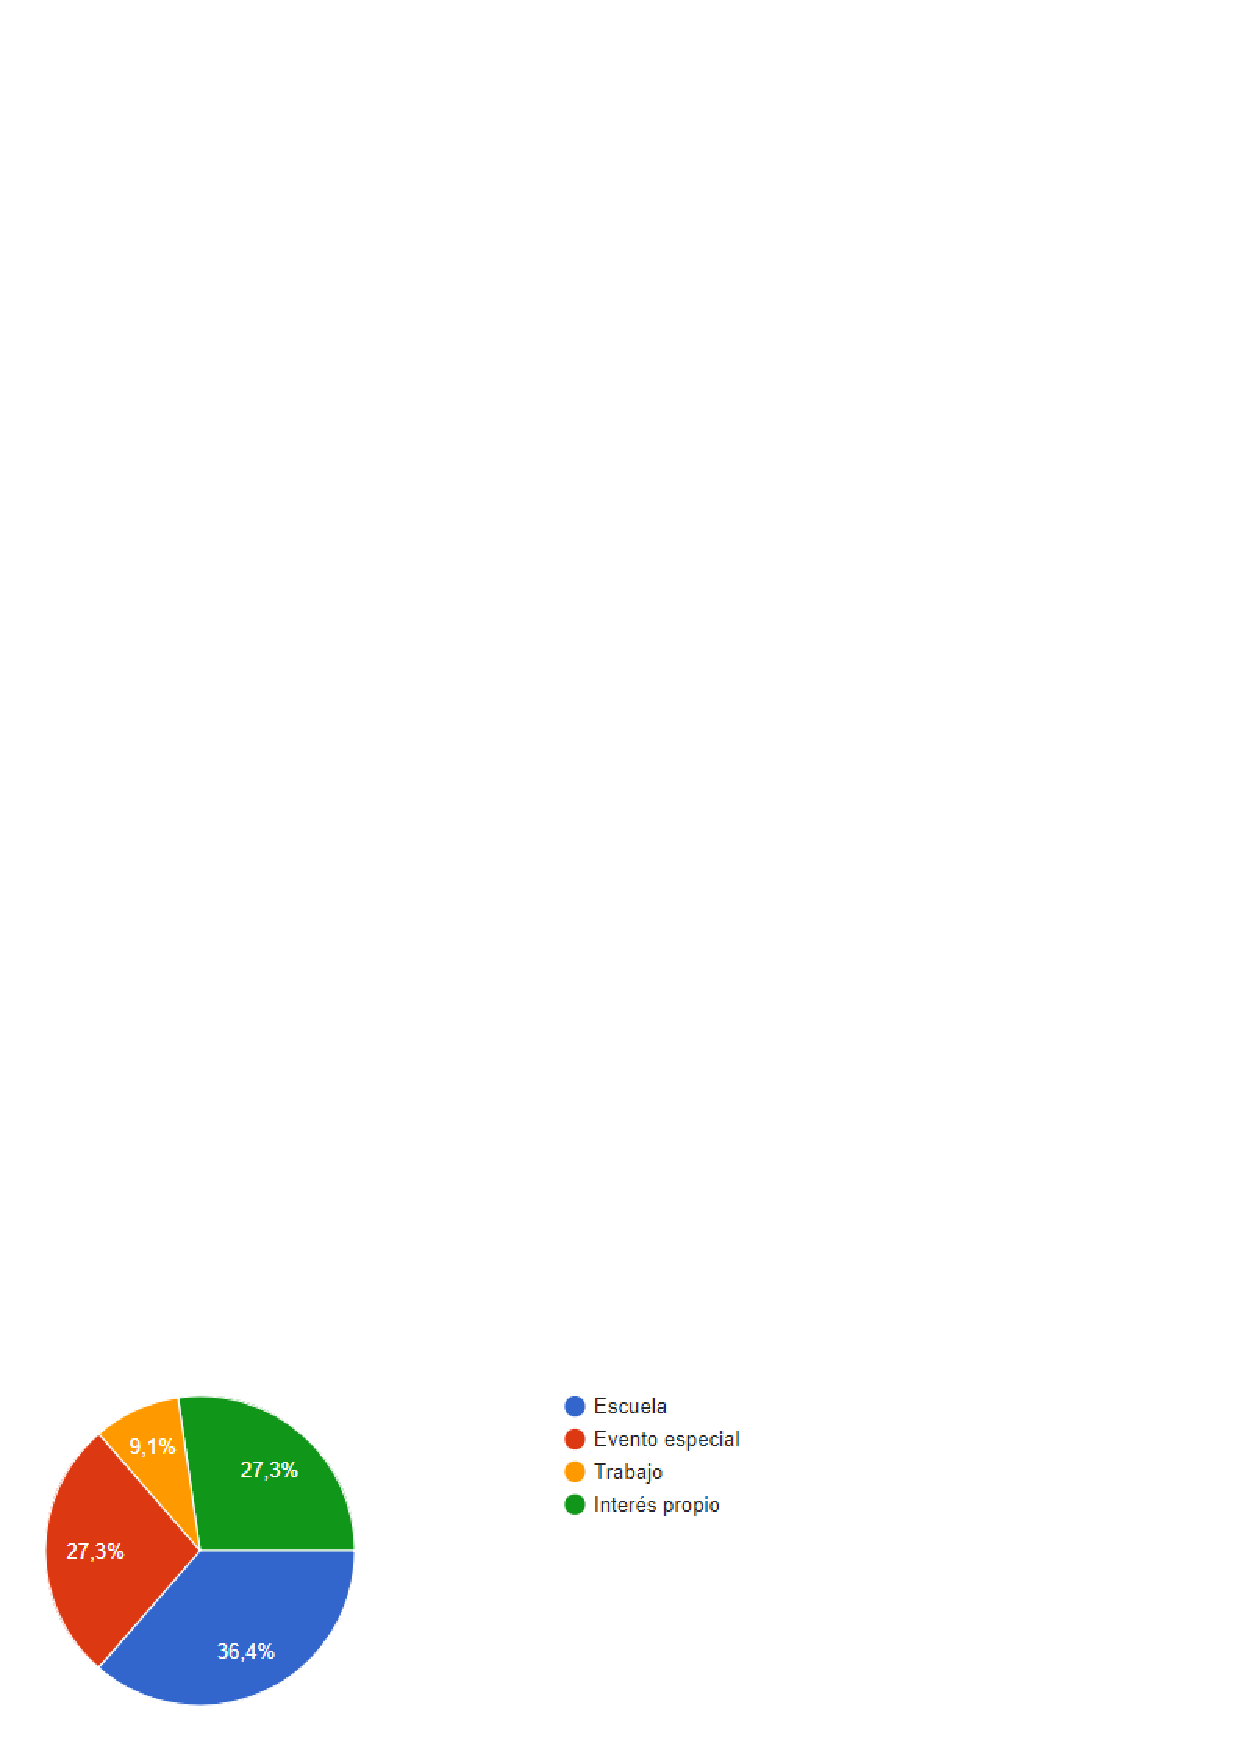
\includegraphics[width=0.5\textwidth]{imagenes\que\pre03}
\end{figure}

	
	\question ¿Sabes sobre la cultura prehispánica en México?
	\begin{checkboxes}
		\choice Sí
		\choice No
		\choice Creo
	\end{checkboxes}

\begin{figure}
	\centering
	\caption{Gráfica de cultura prehispánica}
	\label{fig:pre04}
	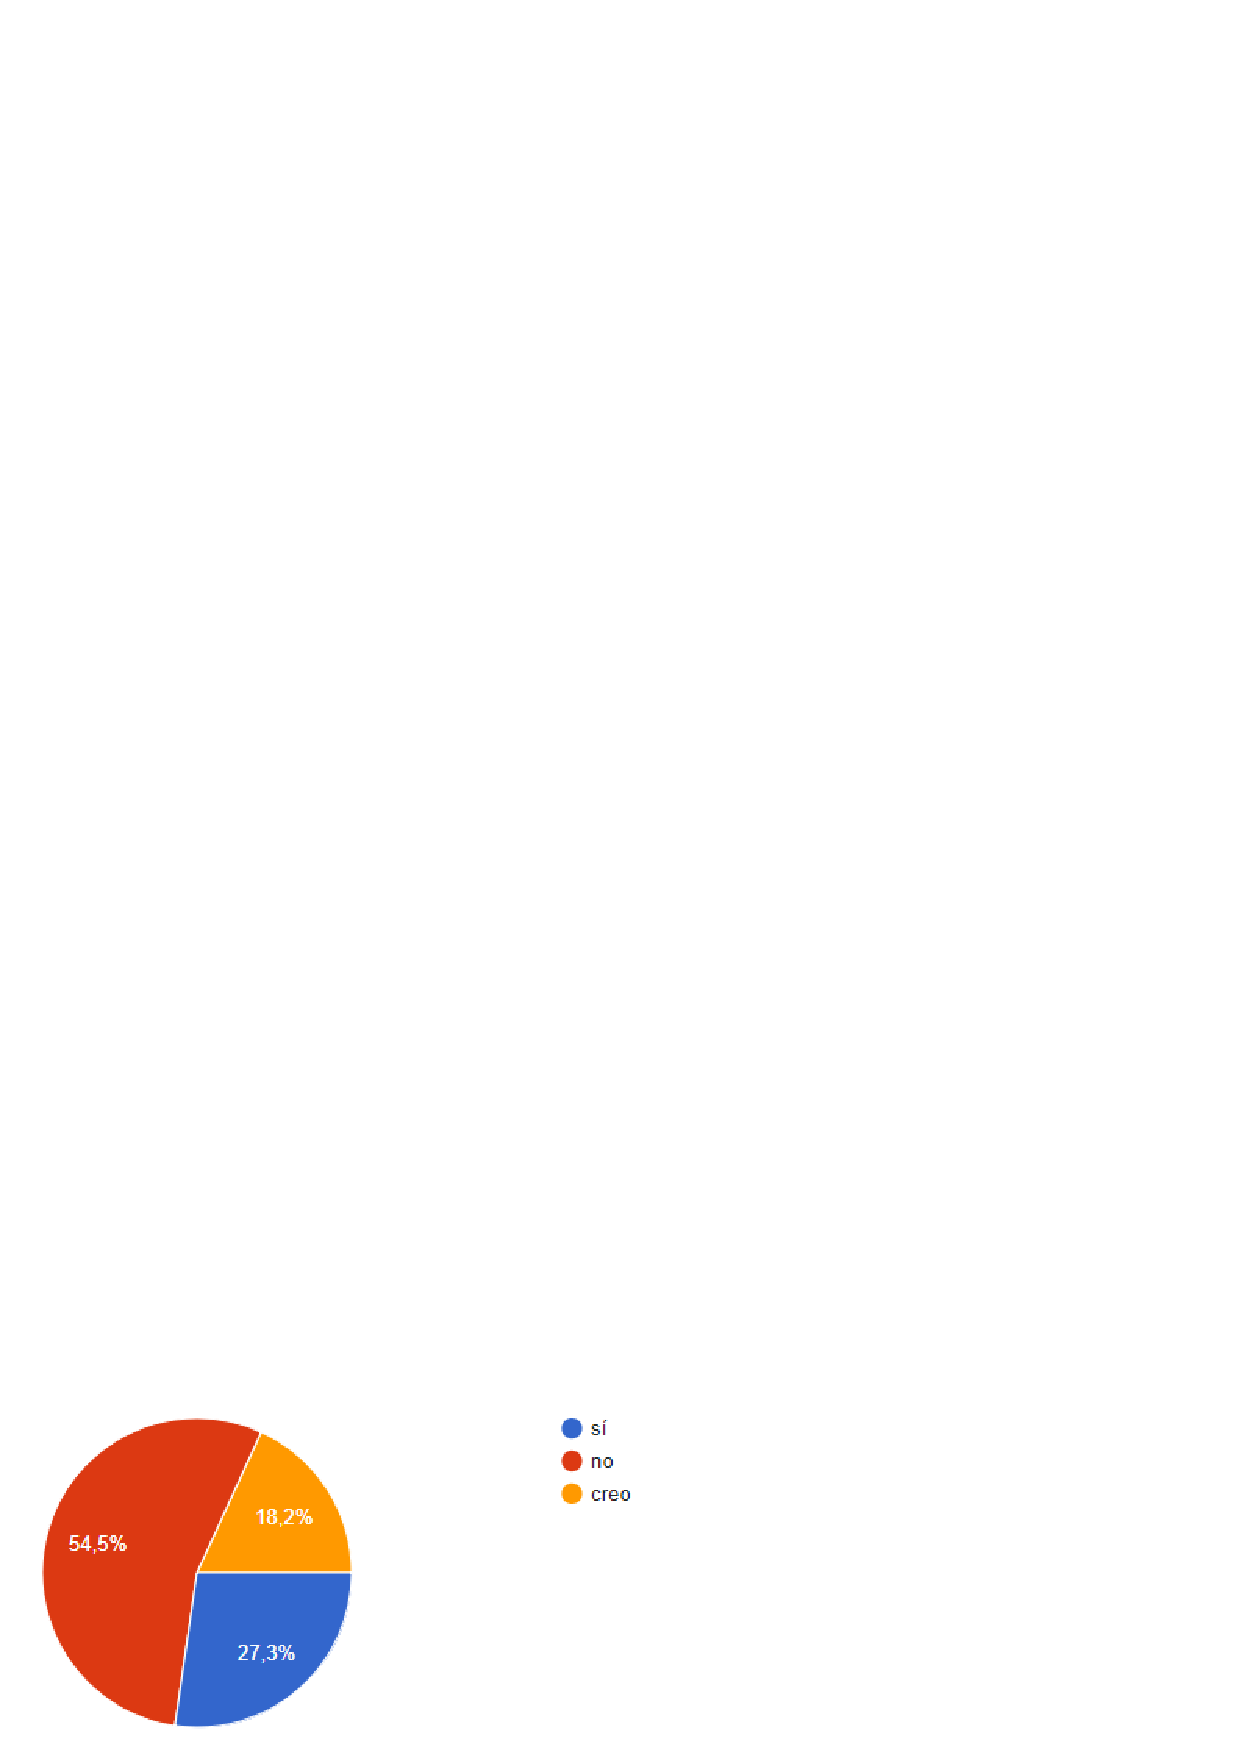
\includegraphics[width=0.5\textwidth]{imagenes\que\pre04}
\end{figure}

	
	\question ¿Qué senitmiento tienes? 
	\begin{checkboxes}
		\choice Alegría
		\choice Enojo
		\choice Tristeza
		\choice Curiosidad
		\choice Fatiga
		\choice Otro? _______
	\end{checkboxes}

\begin{figure}
	\centering
	\caption{Gráfica de sentimiento}
	\label{fig:pre05}
	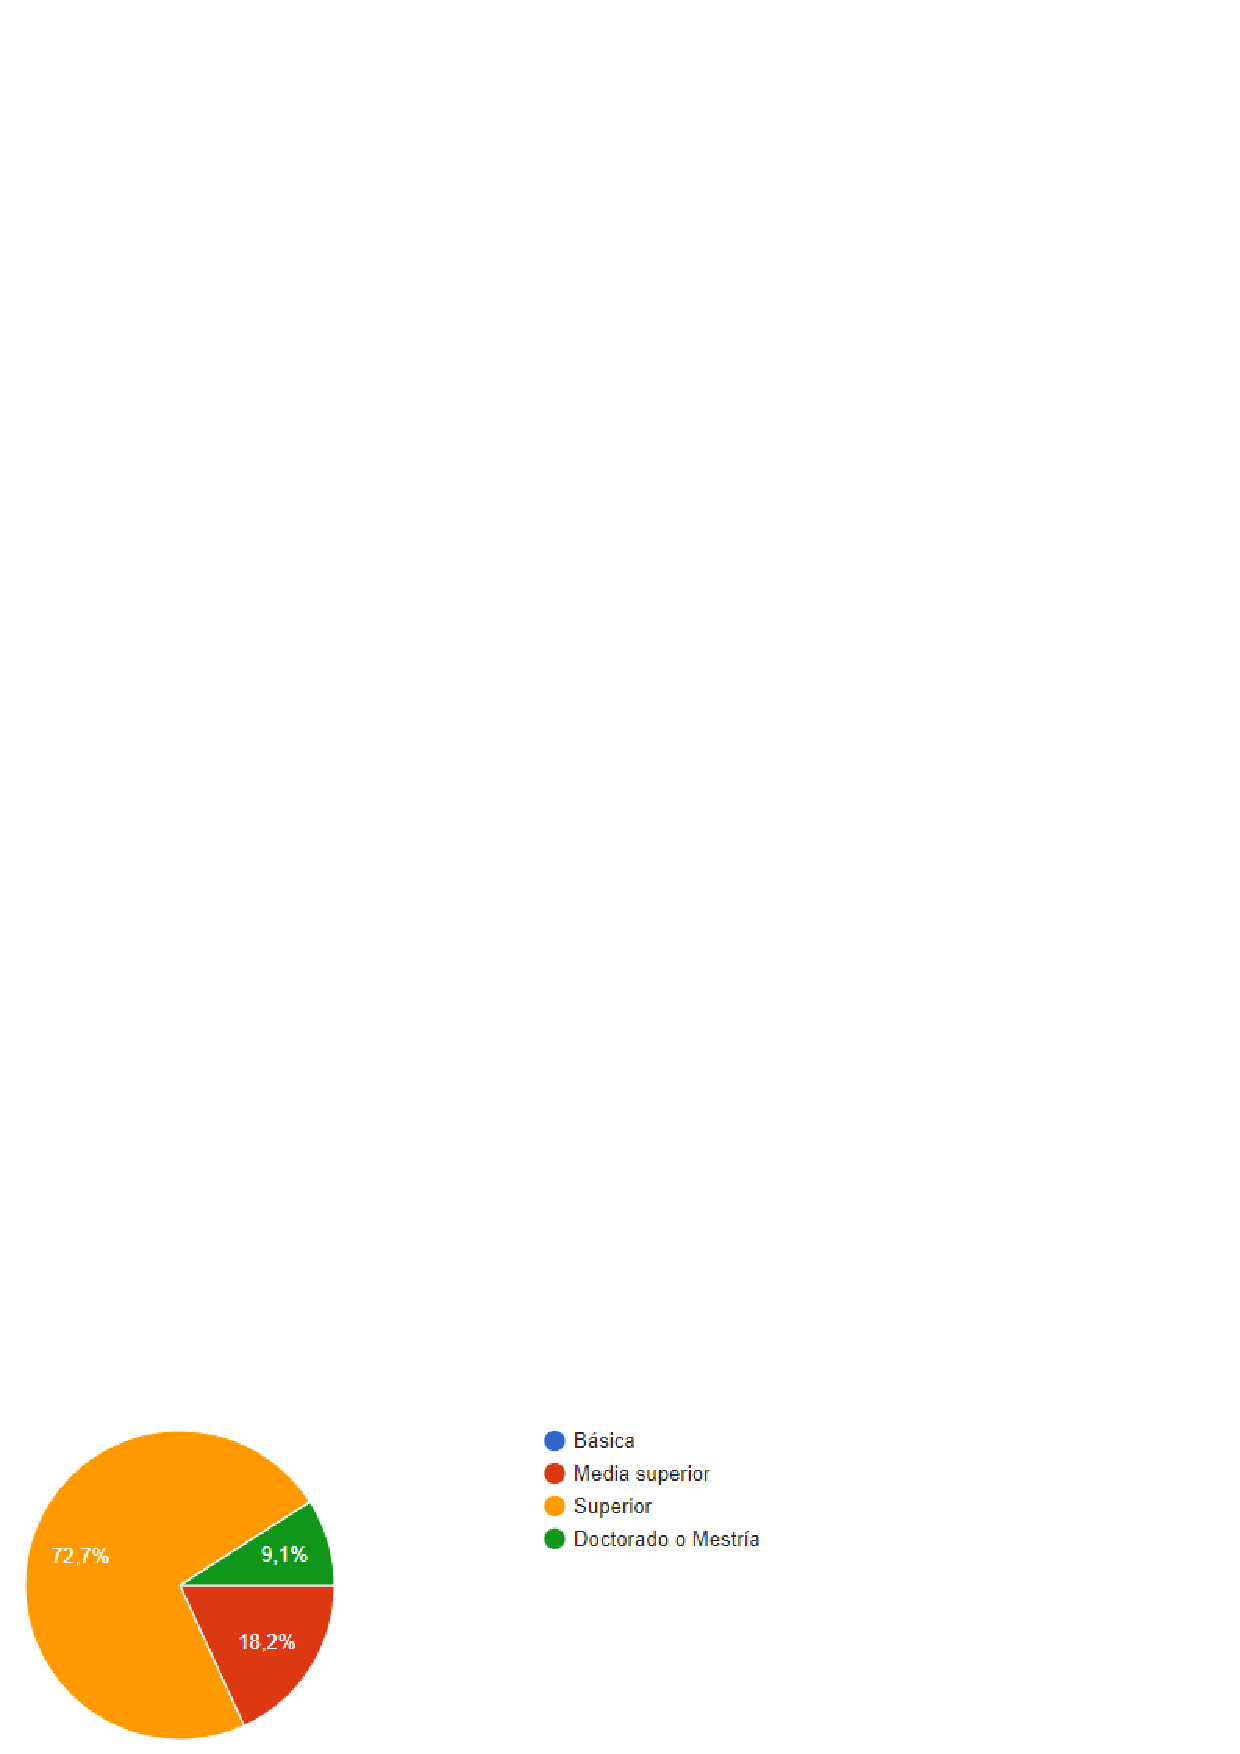
\includegraphics[width=0.5\textwidth]{imagenes\que\pre01}
\end{figure}

	
	\question Pirámide emocional. ¿En que escalón te encuestras ahora?
	%%poner imagen
	La emoción que tenían los encuestados en ese momento era un estado de seguridad o tranquilidad.
	
	
\end{questions}

\subsubsection{Post-juego}
\begin{questions}
	
	{%
	\checkboxchar{$\Box$} % changing checkbox style locally
	\question ¿Hay algún elemento que no reconozcas  o sepas que es?
	\begin{checkboxes}
		\choice Items
		\choice Personajes
		\choice Fondo
		\choice Texto (palabra)
		\choice Lugar
		\choice Tiempo
		\choice Forma
		\choice Otro?
	\end{checkboxes}
}%		

Respuesta: Los encuestados en su mayoría no reconocian diferentes formas o imágenes de objetos presentados en el juego.	

	\question ¿Cómo califica la velocidad de reacción de los botones?
	\begin{checkboxes}
		\choice Mala
		\choice Regular
		\choice Buena
	\end{checkboxes}

\begin{figure}
	\centering
	\caption{Gráfica de velocidad de botoness}
	\label{fig:pos01}
	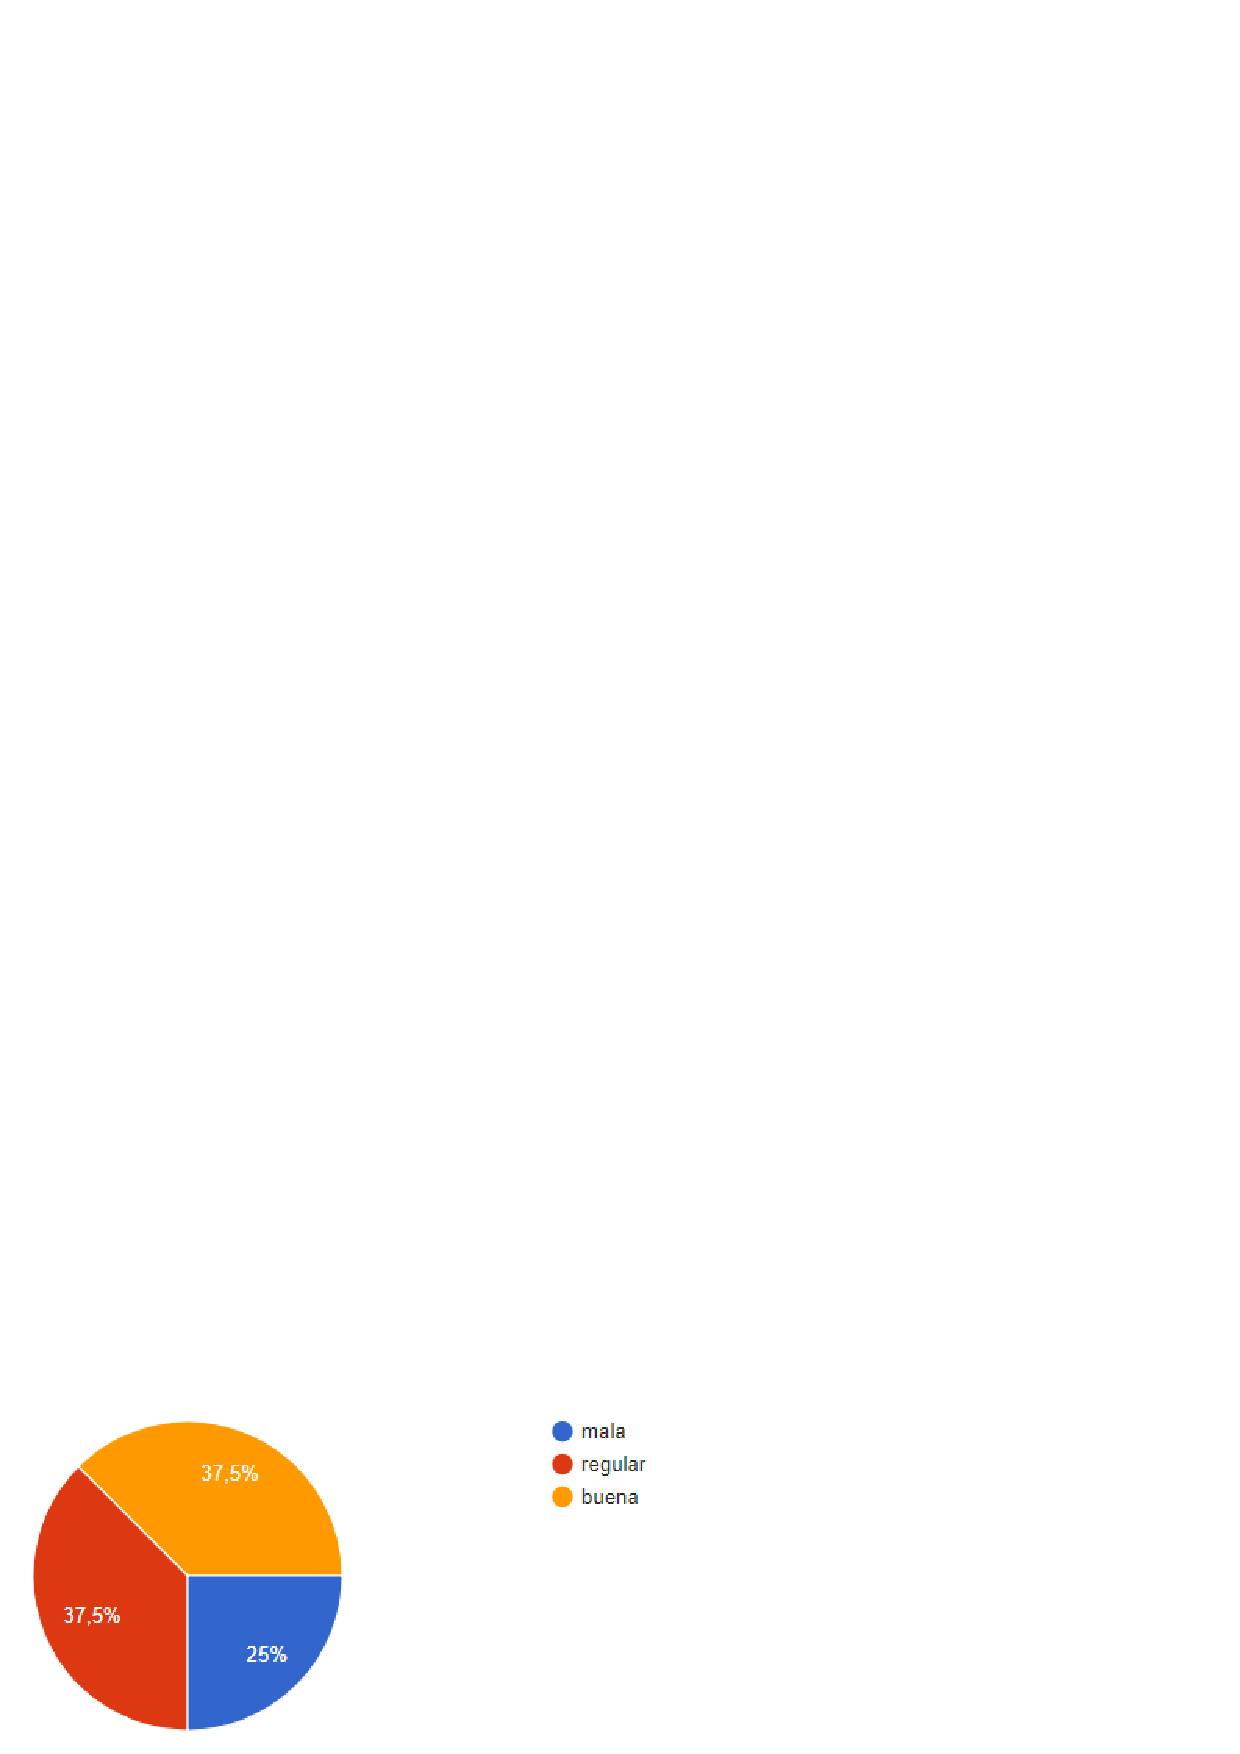
\includegraphics[width=0.5\textwidth]{imagenes\que\pos01}
\end{figure}

	\question ¿Qué te ha gustado MENOS del juego?
	\begin{checkboxes}
		\choice Juego
		\choice Dibujo
		\choice Historia
		\choice Temática
		\choice Plataforma
	\end{checkboxes}

\begin{figure}
	\centering
	\caption{Gráfica de menos gusto}
	\label{fig:pos02}
	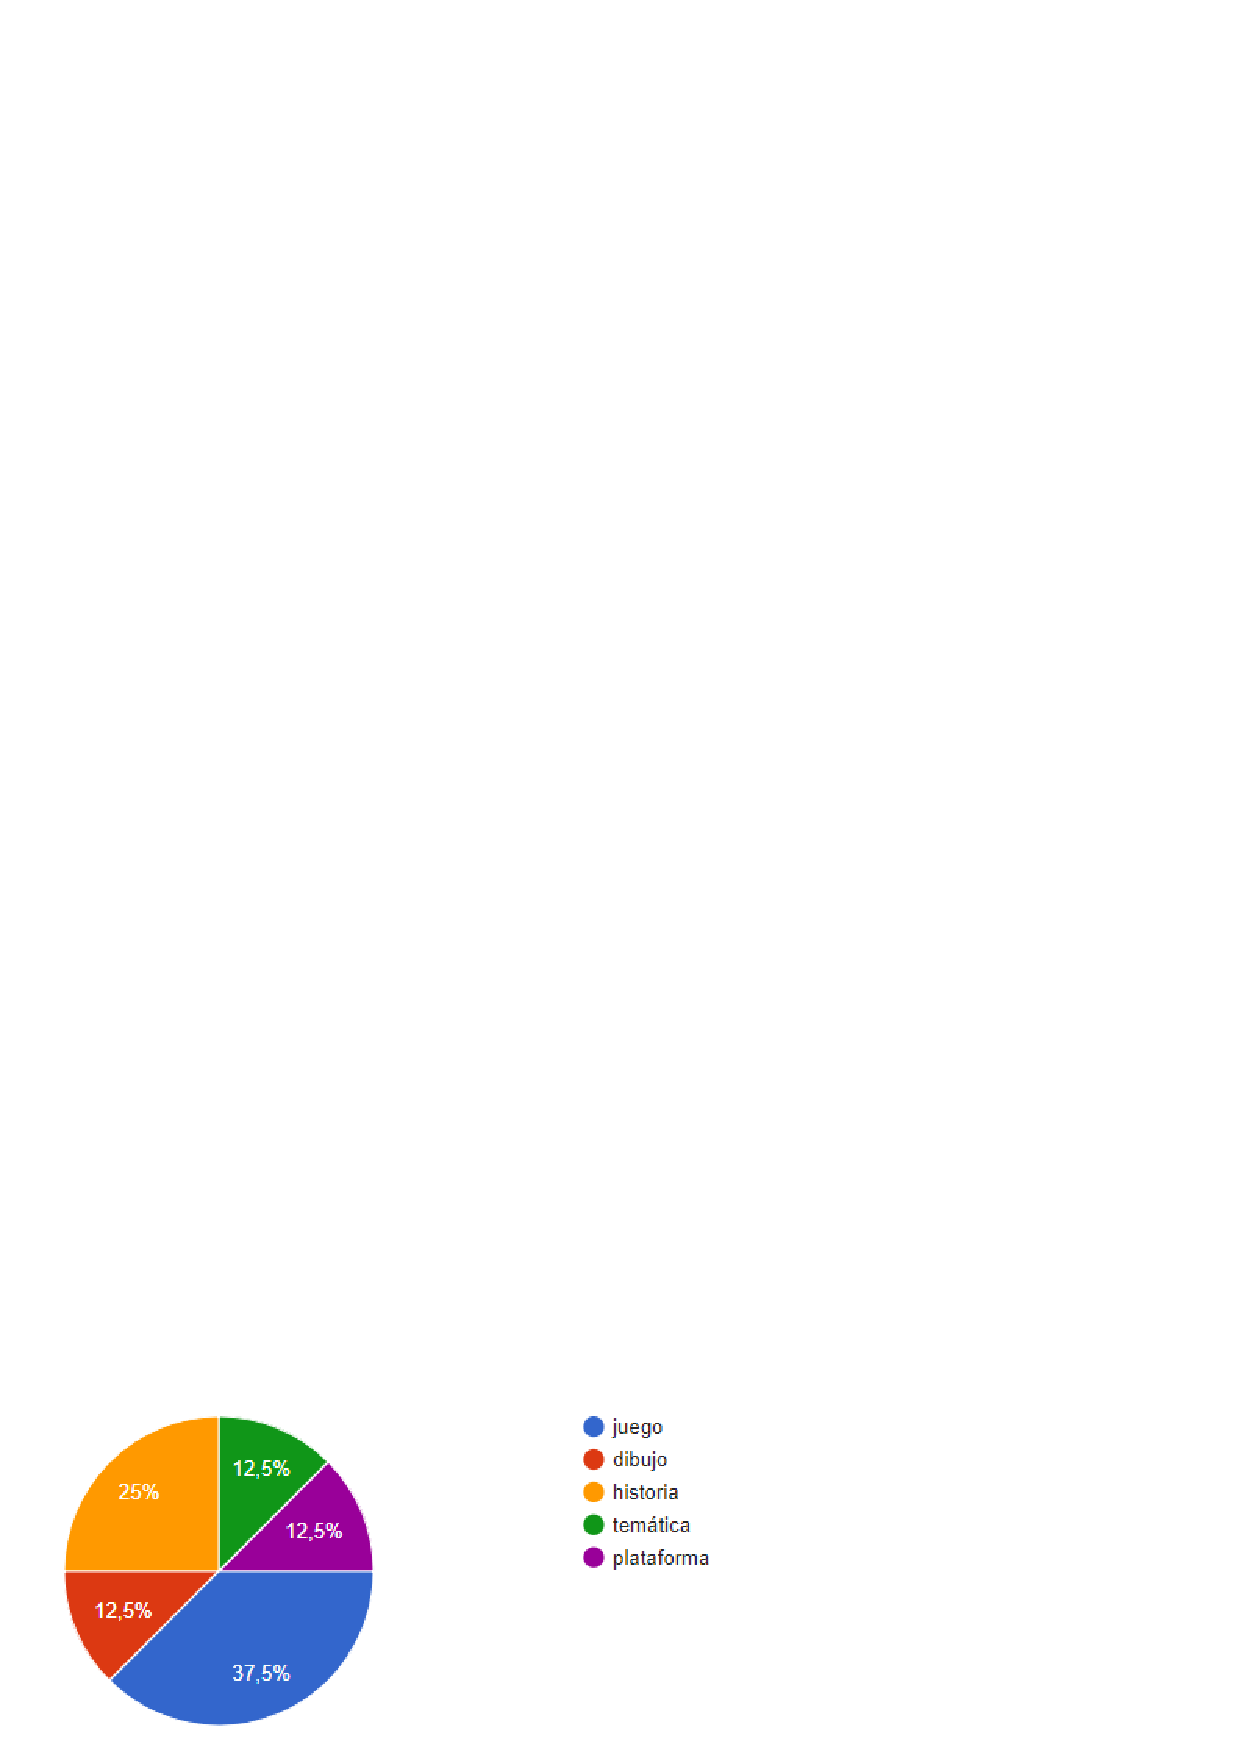
\includegraphics[width=0.5\textwidth]{imagenes\que\pos02}
\end{figure}

	
	\question ¿Qué te ha gustado MÁS del juego?
\begin{checkboxes}
	\choice Juego
	\choice Dibujo
	\choice Historia
	\choice Temática
	\choice Plataforma
\end{checkboxes}

\begin{figure}
	\centering
	\caption{Gráfica de más gusto}
	\label{fig:pos03}
	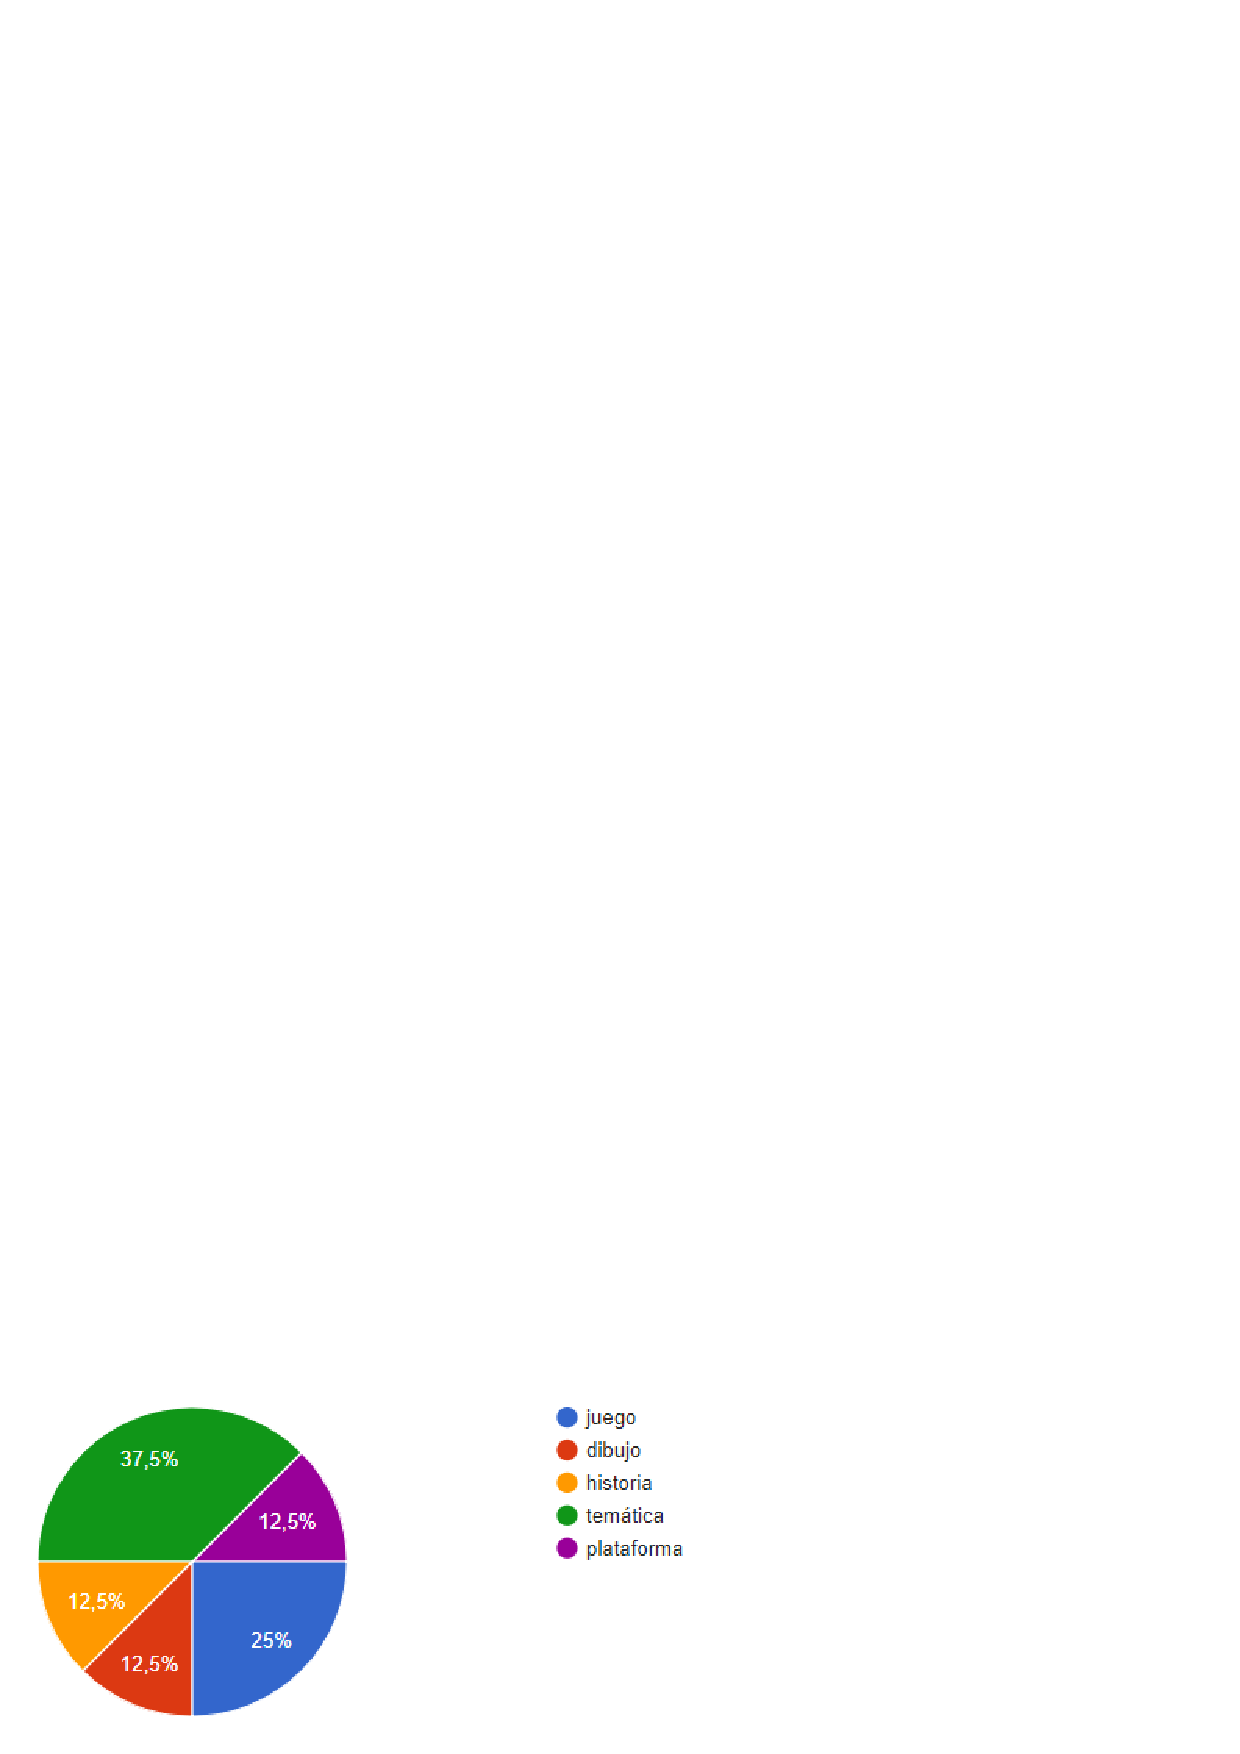
\includegraphics[width=0.5\textwidth]{imagenes\que\pos03}
\end{figure}


	\question ¿Qué dificultad encontraste al jugar?
	_______________________________
	Respuesta: Los encuestados en su mayoría contestaron sobre los movimientos o acciones que se podían realizar dentro del juego, que asu percepción parecían aveces impredecibles.

	\question ¿Que cambiarías del juego?
	______________________________
	Respuesta: Los usuarios en su mayoria mencionan sobre una mayor interacción en el juego sobre el personaje a otras acciones o eventos. 
	

	\question ¿Qué senimiento tienes? 
	\begin{checkboxes}
		\choice Alegría
		\choice Enojo
		\choice Tristeza
		\choice Curiosidad
		\choice Fatiga
		\choice Otro? _______
	\end{checkboxes}

\begin{figure}
	\centering
	\caption{Gráfica de sentimiento}
	\label{fig:pos04}
	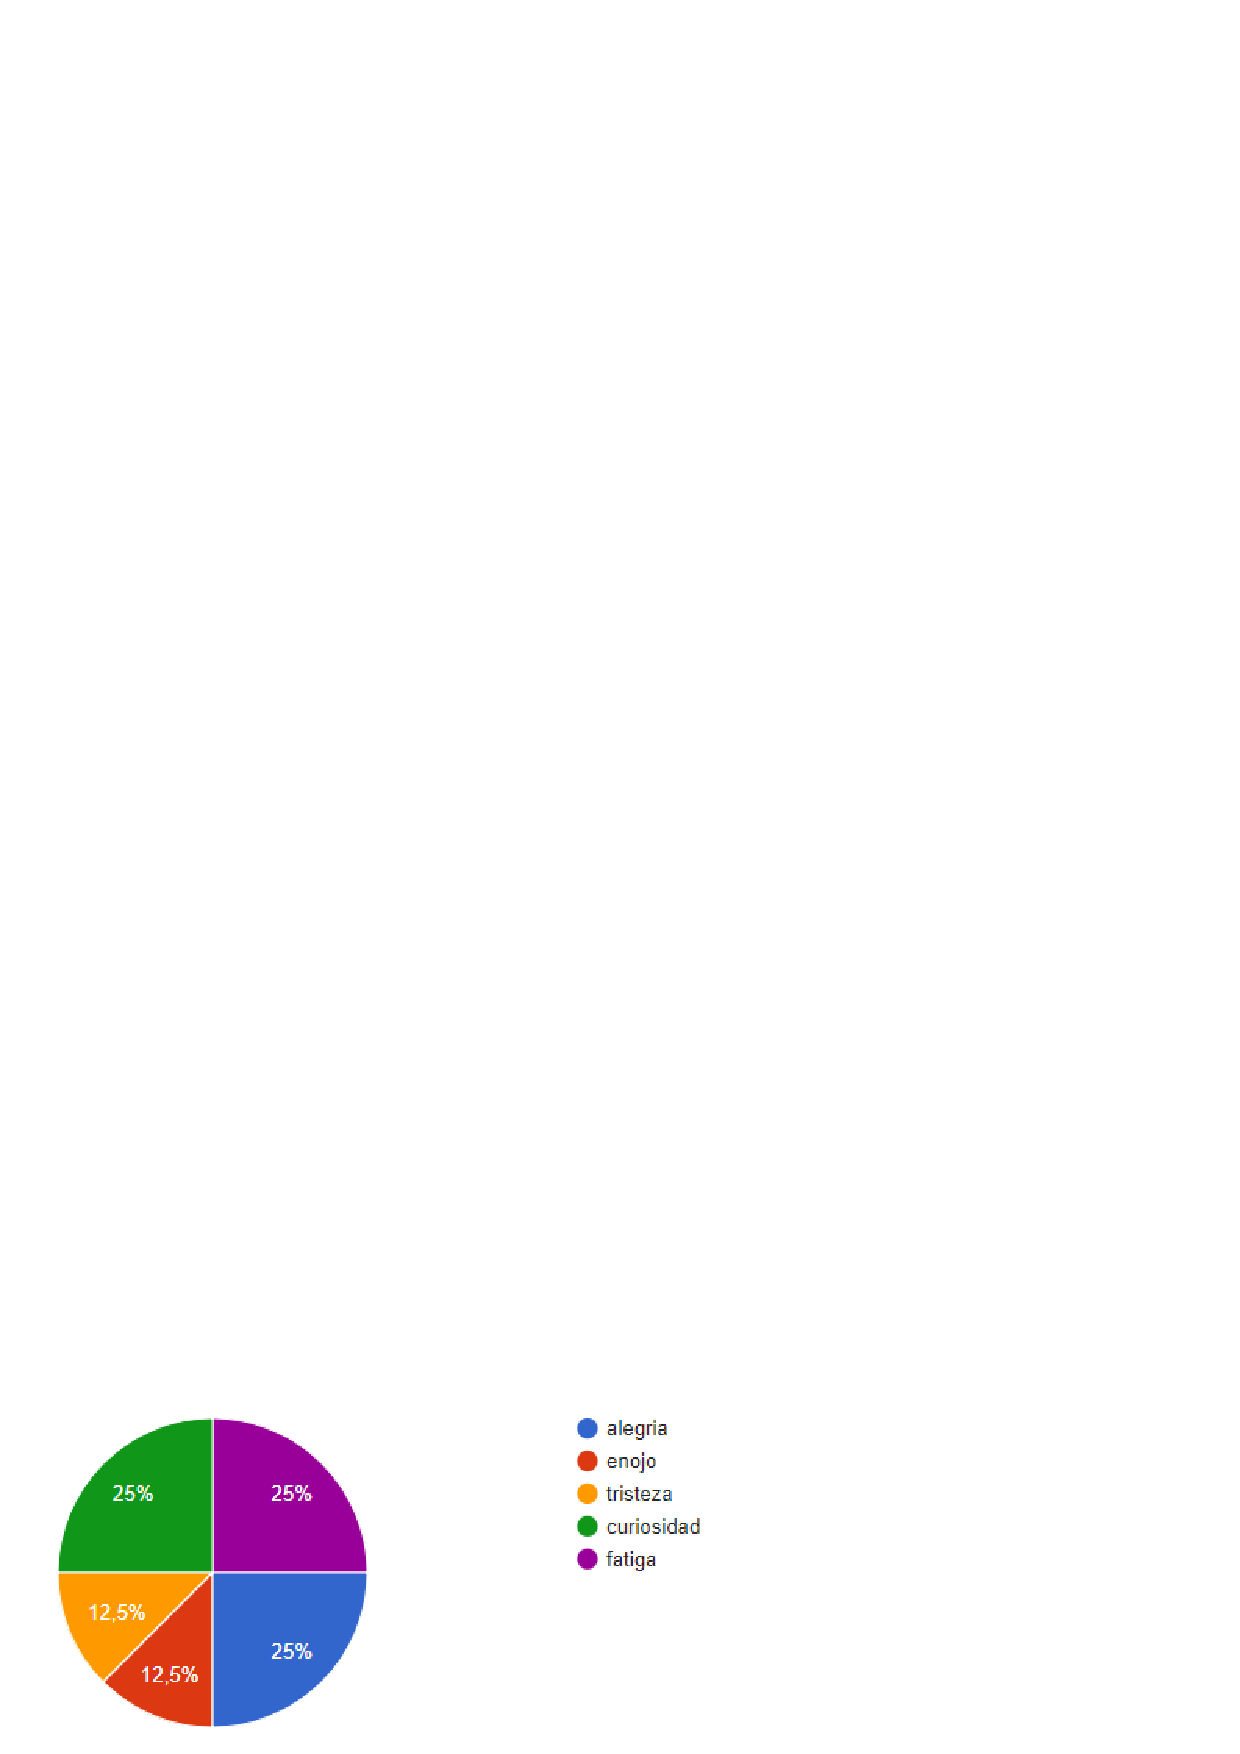
\includegraphics[width=0.5\textwidth]{imagenes\que\pos04}
\end{figure}



	\question Pirámide emocional. ¿En que escalón te encuestras ahora?
	%%poner imagen
	Respuesta: La mayoría de los jugadores seguía en el estado de seguridad o tranquilidad después del juego y seguidos de ellos algunos presentaban una emoción de autorrealización.


\end{questions}

